\section{Improvements ideas}
\label{sec:discussion}
ADOP\cite{ruckert2022adop} is overall an excellent paper. It does not bring so much novel ideas but makes a considerable engineering effort to apply the core idea of NPBG \cite{Aliev2020} to pretty big real scenes.

\noindent \textbf{Only real scenes.}
Suprisingly, the authors do not mention any attempts to apply their method to synthetic scenes, like the NERF paper initially did and they mention that training a new scene requires a large amount of compute. This could mean they developped their method progressively on a few toy examples and didn't bother releasing results of these tiny examples. Or their method may simply not perform too well on synthetic scenes... which may include a lot of specular materials. Classical NERF test samples scenes usually contain a lot of specular materials where the rendering would most probably fail. I still think it would be beneficial to have a few synthetic scenes to test on including to make quick tests without the need of A100 40Gb trained for several hours.
On the other hand, since the main method's contribution are refining pose estimation (requiring the approximate differentiable aspect of the renderer) and the camera photo simulator, it's not surprising that they'd work on natural photos rather than simulation. 

\noindent \textbf{Camera pipeline module.} 
Their analyzis on this part does not look complete in my humble opinion and looks more like a workaround on having scenes shot with auto-exposure. They picked the low hanging fruits: take care of most exposure changes to end up improving the metrics on the available benchmark (Table 4. from their paper shows that ADOP is better by a large margin than all other algorithms except the M60 tanks scene which has been shot in manual frozen exposure). Their claim of bringing novelty and being able to handle the camera imaging pipleine as part of their pipeline may b 

Simulating a realistic camera pipeline (like mimicking the ISP which goes from 12bit linear RAW bayer data to a 8 bit jpg) is probably as difficult as correcting first order errors introduced by the camera's ISP as part of the optimization process...Despite the effort on the ablation study (table 3 and figure 6 of \cite{ruckert2022adop}), problem is that we don't really know the exact impact of compensating the camera photo pipeline on the final reconstruction result, at least compared to a scene imaged with perfect ideal linear HDR camera. For instance, they're able to get a sky with cyan shift which looks like the camera picture (they fit the tone mapper correctly).

If we carefully look at the Tanks and Temples dataset \cite{Knapitsch2017TanksAndTemples}, pictures are frames extracted from a mp4 video from 2 different high end cameras, sometimes using auto-exposure. Although it's a good initiative for researchers to keep on using fixed established benchmarks, Tanks and Temples was initially designed for 3D reconstructions (e.g. evaluate performances of Structure from motion like COLMAP estimation compared to a groundtruth lidar captured point cloud) rather than novel view synthesis. The idea is interesting but it will most probably fail with a modern smartphone camera which use local tone mappers and sometimes adapt colors locally.

\label{sec:remplementation}
\begin{figure}[H]
    \centering
    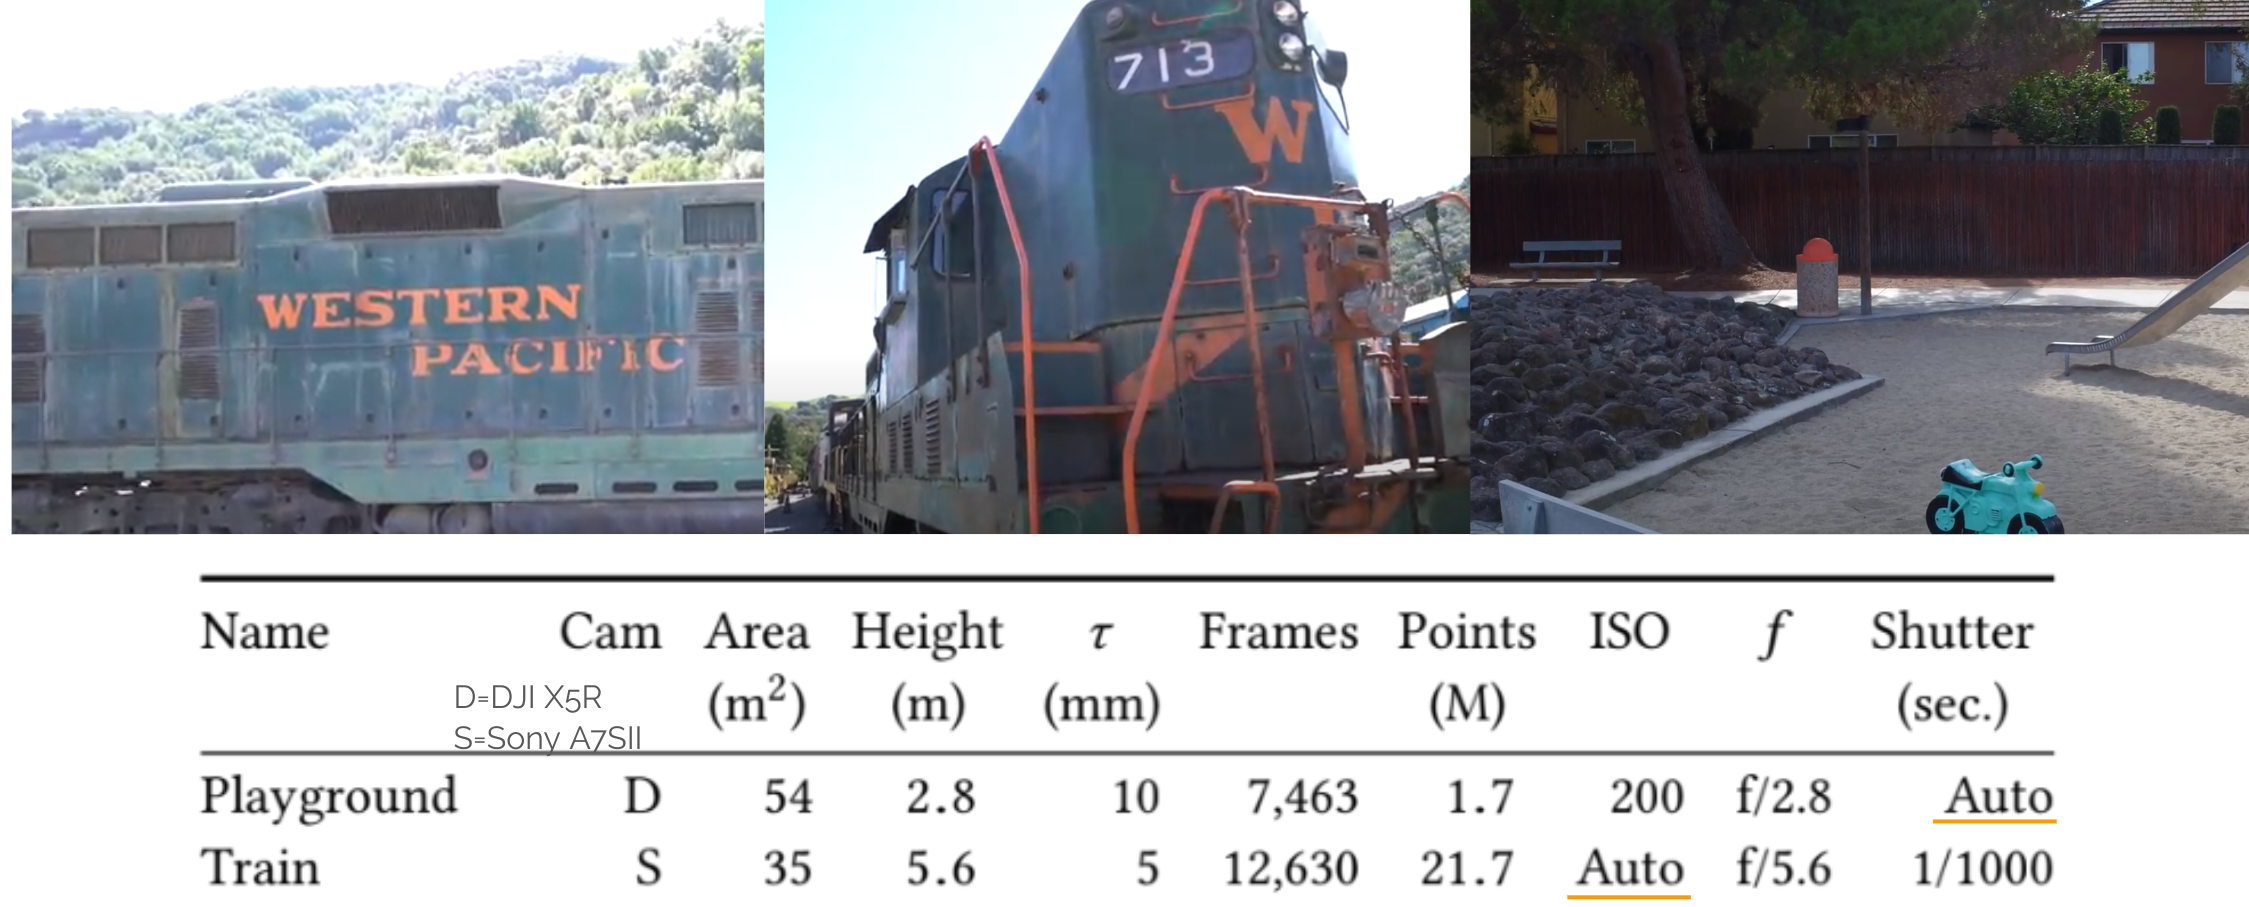
\includegraphics[width=6cm]{figures/tanks_and_temples.png}
    \caption{Information on the scenes captured for the Tanks and Temples dataset with high end video cameras in addition to a Lidar point cloud. On the left, the "train" scene shows clear signs of overeposure. The playground scene on the right has an overall correct and steady exposure}
    \label{fig:tank_and_temples}
\end{figure}

One of the potential way of creating a new benchmark would be to capture the scenes with a DSLR (like a full frame sensor) shot both in RAW and jpg (usually available on most cameras). RAW files would be post-processed by LightRoom or DxO Photolab with a neutral rendering: no tone mapping and neutral color rendering to get a Linear RGB set of images. HDR could be achieved by bracketing. and serve as the ground truth for validation, without any image compression. Training images would be either the jpgs or the reprocessed RAW files using a more aggressive rendering: vibrancy to make some colors slightly more saturated (e.g. blue for skies but avoid too red skin tones), tone mapping (global or local), sharpening / micro contrast.
